%! Author = Adham Aijou
%! Date = 23.02.2023
\subsection{Use Case}
Hierzu wurde ein Use Case erstellt, welcher die Anforderungen an das System beschreibt.
Dieser Use Case wurde in einem Tabellenformat erstellt, welches in der folgenden Tabelle dargestellt wird:
\newline
\begin{tabularx}{\textwidth}[b]{|l*{2}{|X}|}\hline
    \caption{Use Case - Terminbuchung}
    \label{tab:Terminbuchung}
    Use Case & Ressourcen- und Terminplanung in Office365 mithilfe von Microsoft Graph API\\

    Titel & Finde freie Termine in einem Kalender für eine bestimmte Ressource\\
    \hline
    Beschreibung & Der Benutzer möchte einen Termin in einem Kalender für eine bestimmte Ressource finden.\\
    \hline
    Akteure & Benutzer, Ressource, Kalender\\
    \hline
    Vorbedingungen & Der Benutzer ist angemeldet.\\
    \hline
    Nachbedingungen & Der Benutzer hat einen Termin in einem Kalender für eine bestimmte Ressource gefunden und/oder hat einen Termin gebucht.\\
    \hline
    Normaler Ablauf & \begin{enumerate}
        \item Der Benutzer geht zu einem Tablet, welcher vor dem Raum angebracht wurde, welcher die Ressource stellvertretend repräsentieren soll.
        \item Der Benutzer sieht die verfügbaren Zeiten für die Ressource und den jetzigen Status der Ressource.
        \item Der Benutzer wählt einen Termin aus.
        \item Der Benutzer bucht den Termin.
        \item Der Benutzer erhält eine Bestätigung oder eine Fehlermeldung.
    \end{enumerate}\\
    \hline
\end{tabularx}
\newline
\newline
Dazu gibt es auch ein Diagramm, welches den Ablauf des Use Cases beschreibt:
\newline
\newline
\par\vspace{1cm}
\centering
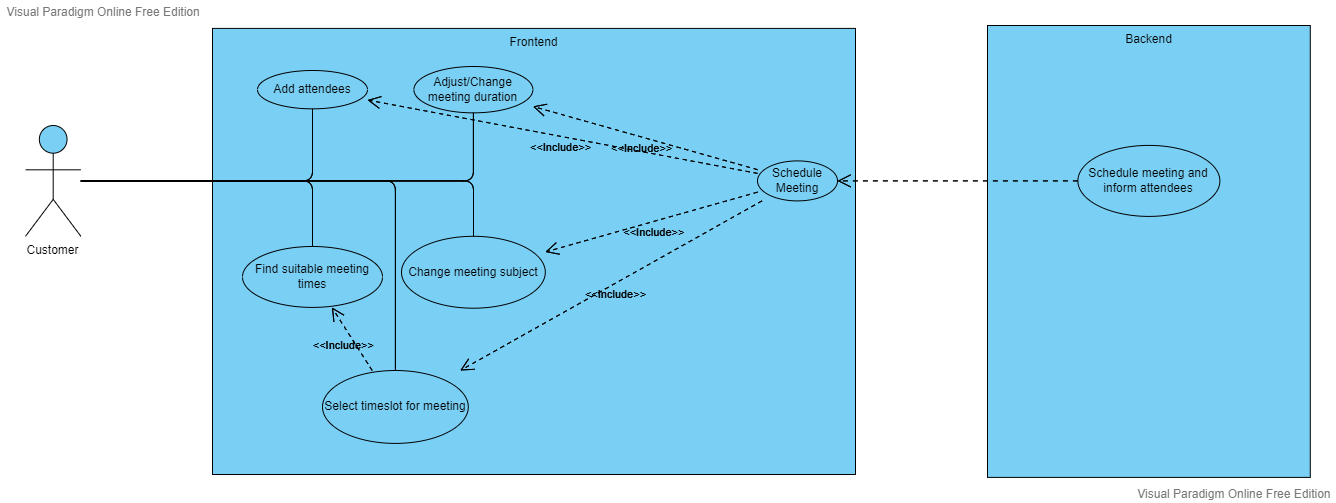
\includegraphics[width=\textwidth]{Bilder/Objektorientiertes Design/Use Case diagram ressource booking}
\raggedright
\newline
\newline
